\section{Anticipating one's own changed options}
\label{sec:finance}

A debt gives planning a known target: raise a stated sum from a menu that changes after each action, or declare bankruptcy. We first ask how demanding the debts were, then examine those where the first menu hides what payment requires.

\subsection{Most debts were easy}
Agents pay 128 of the 188 debts that reached a liquidation menu (Table~\ref{tab:tiers}). Fifty-six of the 60 eliminations owe more than the debtor's own assets could raise. One more, Opus in G7, is within the bound, but the bank has no houses left and the menu offers no building sale; the funds it can reach are \$440 against \$750. The remaining three were payable, as earlier engine-executed sequences showed. Payment therefore succeeds in 128 of 131 debts known to be payable.

\begin{table}[t]\centering\small
\begin{tabularx}{\linewidth}{@{}lYrrr@{}}\toprule
Tier & What the first menu and holdings imply & Episodes & Paid & Declared\\\midrule
\rows{sections/generated/tier_rows}
\bottomrule\end{tabularx}
\caption{All 188 liquidation episodes, classified at the first debt menu. Tiers A, B and N are the 131 payable debts. ``Declared'' means the debtor declared bankruptcy or was eliminated. The three payable declarations rely on inherited engine-executed payment sequences, and the G7 restriction on an inherited menu search.}
\label{tab:tiers}\end{table}

That rate says little about difficulty. In 62 payable debts the cash and listed mortgages suffice, and all are paid. Sixty-seven payments take one action, and the median debt is 36\% of the own-asset bound. Because the menu refreshes after every action, an agent that keeps choosing listed financing actions never has to look ahead to make progress. The decision that needs foresight is whether to stop: bankruptcy is always on the menu, and an agent that judges payment impossible can end its game while a route exists. That judgment matters most in tier N.

\subsection{Sixteen debts that needed released collateral}
In sixteen debts, cash plus every listed mortgage plus the salvage value of every building still falls short. The difference can come only from mortgaging deeds whose buildings must first be sold. Figure~\ref{fig:necessary} shows each case. Agents pay fourteen. Gemini pays five of six, Opus five of five, Sol two of three and Grok two of two. The amount that only released collateral can supply ranges from \$12 to \$326.

\begin{figure}[t]\centering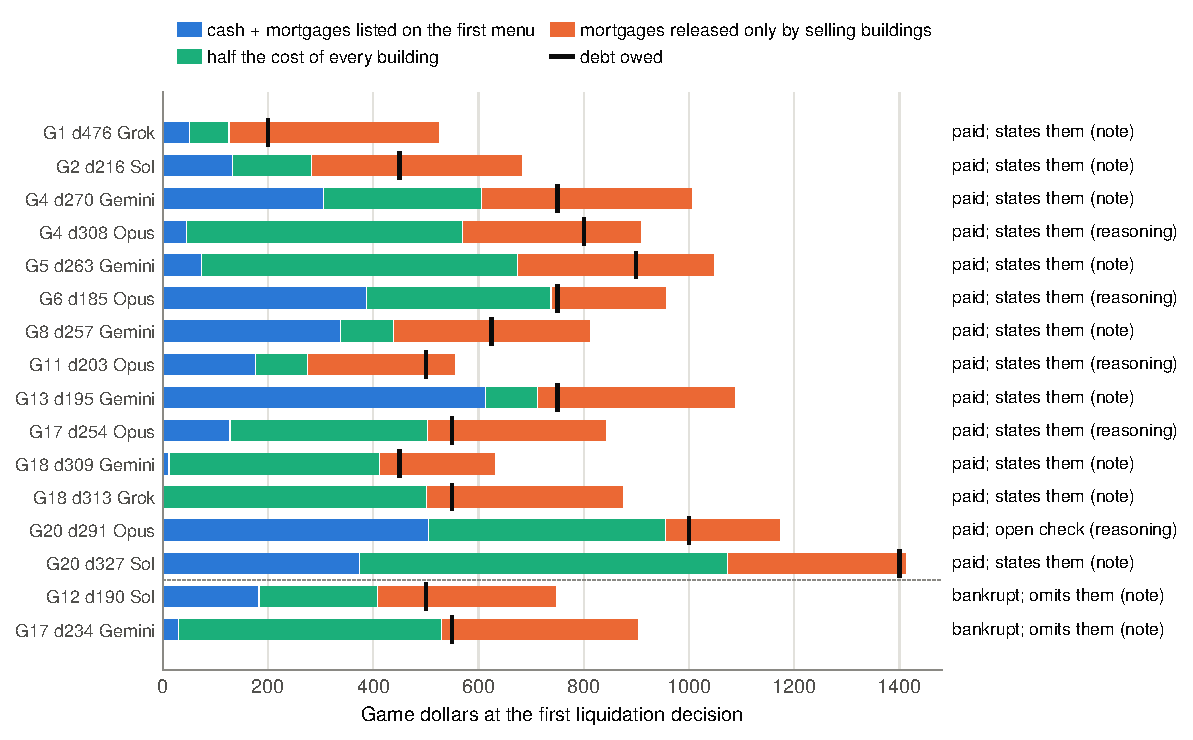
\includegraphics[width=\linewidth]{necessary_collateral.pdf}
\caption{The sixteen debts in which payment required mortgages released only by selling buildings. Each bar stacks what the debtor could see at the first menu (blue), the salvage of every building (green) and the mortgages that sales would release (orange); the black tick is the debt. Right labels give the outcome and our single-reader classification of the first-decision text (states the released mortgages, raises them as an open check, or omits them), with its channel (applied note or provider-returned reasoning). Opus texts are provider-returned reasoning under action-only recovery; all others are applied private notes. Numbers are in Appendix Table~\ref{tab:necessary}.}
\label{fig:necessary}\end{figure}

We read the recorded text at each first decision, before any action in the episode was applied. In thirteen of the fourteen payments the text names the mortgages that sales will release, or states a budget that includes them. Nine of these are applied private notes from Sol, Gemini and Grok. Four are Opus's provider-returned reasoning; under recovery Opus wrote no note. Grok's note at G1 d476 is typical: \emph{``\InlineQuote{nec-g1-d476}''} In the fourteenth payment, Opus at G20 d291 correctly finds that listed items leave it short and then writes, \emph{``\InlineQuote{nec-g20-d291}''} It goes on to pay.

The stated figures are mostly correct. In twelve of the thirteen explicit texts, every stated amount matches the board and the delivered state. Sol at G2 d216 values the released yellow mortgages at \$430 when they total \$400, which still covers its \$167 gap. Gemini at G4 d270 and G8 d257 names the released mortgages without valuing them. One text shows the step being made. Gemini's returned reasoning at G5 d263 first totals only the house sales, then writes that the deeds can be mortgaged after the houses are sold, and its applied note gives the correct total of \$1,049.

Both bankruptcies follow notes that add up only what the first menu lists. Sol at G12 d190 writes, \emph{``\InlineQuote{nec-g12-d190}''} It omits \$340 of red mortgages that its own sales would release, and declares. Gemini at G17 d234 counts \emph{``\InlineQuote{nec-g17-d234}''} and omits \$375 of dark-blue mortgages. Neither applies any action before declaring. Both systems pay other tier N debts, so the omission is a lapse in particular states rather than a fixed property of either system.

These episodes reach \Level{accurate} and \Level{consistent}: the stated dependency matches the rules and state, and the actions carry it out. In the two failures an inaccurate total is followed by the action it implies. The texts do not show how the systems computed, the sixteen cases were identified after the corpus had been studied, and they contain only two failures. A policy that never declares while a financing action is listed would avoid both failures by construction; whether it would always reach payment under the even-sale and bank-stock rules we did not test.

\subsection{What the sequences ask of the agent}
The fourteen paid tier N sequences take two to ten actions. Each sells buildings before its first released mortgage and needs one kind of prerequisite: clear a group's buildings evenly, then mortgage the group. Execution length therefore overstates dependency depth, and since refreshed menus show each released mortgage once it exists, the actions could follow from step-by-step feedback. The first-decision text adds a prospective statement of a resource the first menu does not show.

Released collateral is used more widely than it is needed. Nineteen payments use 33 mortgages absent from the first menu. Fourteen are the necessary cases. In the other five, four by Gemini in G3 and one by Sol in G18, the agents could have paid from listed mortgages and salvage alone.

\IncidentTitle{g20pay}{A ten-action liquidation reaches its stated remainder}
In G20 only Gemini and Sol remain. Sol has \$49, nine orange houses and two brown hotels. Before raising Pennsylvania Avenue's rent to \$1,400, Gemini values its rival's estate:
\TranscriptQuote{g20-creditor}
Sol lands there on the next turn. Its note at the first liquidation decision states an aggregate budget and one ordering constraint:
\TranscriptQuote{g20-plan}
Sol sells its development in two actions and mortgages eight deeds, five of them released by the sales. At the last mortgage it writes:
\TranscriptQuote{g20-last}
The events record \$700 from sales and \$665 from mortgages, so \$49 + \$700 + \$665 $-$ \$1,400 = \$14. Gemini's total is also right, but its parts are not: it books \$675 of salvage and \$690 of mortgages, two errors of \$25 that cancel. Sol's budget is the stronger evidence because the actions that follow confirm it. The note specifies a total and a rule for hotel sales, not an ordered list of ten actions; the menus supplied the order. This incident reaches \Level{accurate} and \Level{consistent} for both the debtor's plan and the creditor's total, with the creditor's components inaccurate.
\TranscriptSource{G20 d325 and d327--336, standard prompt. All three quotations are private notes and were not delivered to the other player. Amounts are from turn-108 events.}

\paragraph{A different kind of failure.} The third payable declaration has another cause. At G12 d249 Grok owes \$250 with \$43 cash and seven pink houses. Its applied note first concludes that payment is impossible, then recomputes and ends, \emph{``\InlineQuote{g12-note-inline}''} Its assistant content names a two-house sale. The received call declares bankruptcy, with the public message ``\InlineQuote{g12-public-inline}'' The engine applies the call. The note and the assistant content agree with each other, and the applied call contradicts both. We count this case as a channel conflict and do not treat it as an omission of collateral.
